% !TEX root=../main.tex
\documentclass[beamer]{standalone}
\begin{document}
% ==============================================================
% Method : Gradient Descenet Explanations - 0 
% ==============================================================   
\begin{frame}{Method}
    \framesubtitle{Result: Gradient filtering on a texture - bug}
        \begin{figure}[t]
            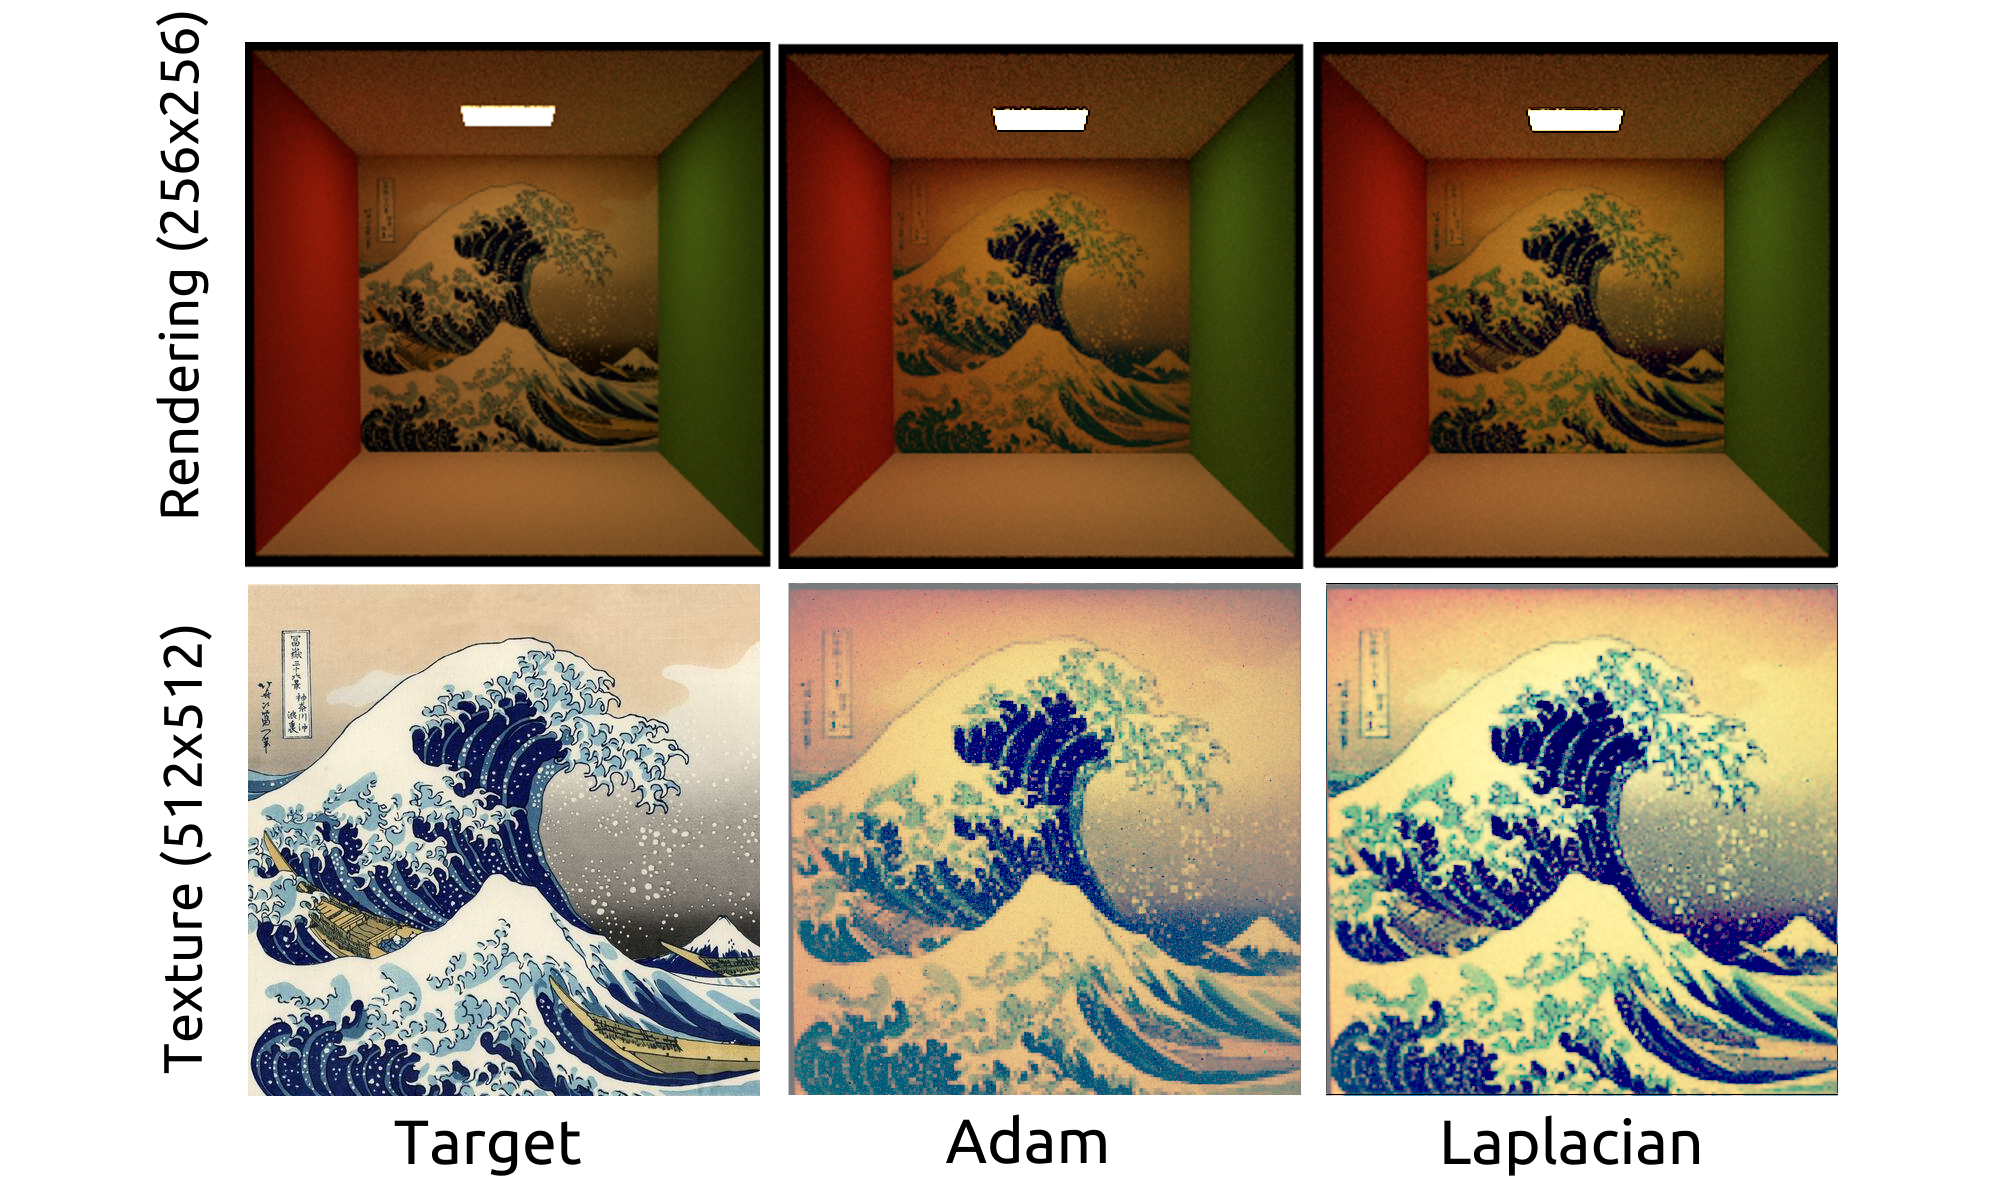
\includegraphics[width=6cm]{./figures/result-1.png}
        \centering
        \end{figure}
        \begin{itemize} 
            \item Currently, code has the bug
            \item MSE records
            \item learing rate: 0.5
        \end{itemize}
        \begin{table}
            \centering
            \resizebox{12cm}{!}{
            \begin{tabular}{ | c | c | c | c | c | c | c | c | c | c | c | c } \hline
                iter     & 1      & 2      & 3      & 4      & 5      & 6      & 7      & 8      & 9      & 10     \\\hline
                filter   & 0.1017 & \alert{0.0792} & 0.0625 & 0.0515 & 0.0462 & 0.0431 & 0.0412 & 0.0400 & 0.0393 & 0.0388 \\ \hline
                No       & 0.1016 & \alert{0.0912} & 0.0824 & 0.0752 & 0.0695 & 0.0650 & 0.0613 & 0.0584 & 0.0560 & 0.0540 \\ \hline  
            \end{tabular}}
        \end{table}
    % note %
    \note[item] {
    }
\end{frame}

% ==============================================================
% Method : Gradient Descenet Explanations - 1 
% ============================================================== 
\begin{frame}{Method}
    \framesubtitle{Result: Gradient filtering on a texture, Weigthed Gaussian Kernel version}
        \begin{figure}[t]
            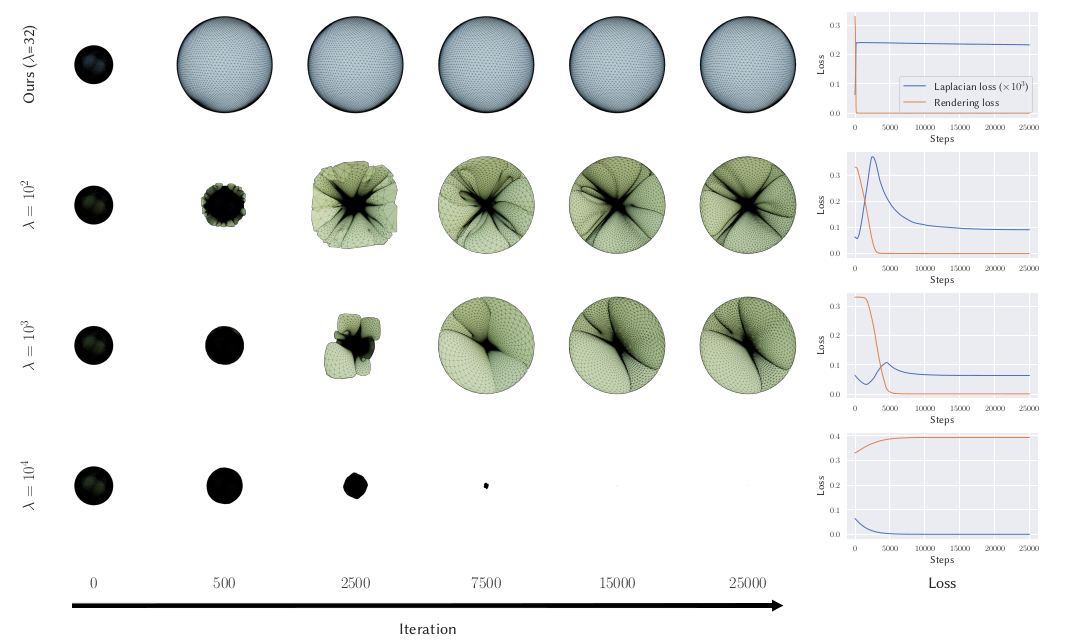
\includegraphics[width=6cm]{./figures/result-2.png}
        \centering
        \end{figure}
        \begin{equation}
            x \leftarrow x - \eta {(w*(D^{-1}G(x, \sigma)-D))}{\diffp{\Phi}{x}}
        \end{equation}
        \begin{itemize} 
            \item Whatever the laplacian operator is, if we want to filter the gradient, 
            the directly multiplying kernel reduce noise and weight give more step length
        \end{itemize}
        \begin{table}
            \centering
            \resizebox{12cm}{!}{
            \begin{tabular}{ | c | c | c | c | c | c | c | c | c | c | c | c } \hline
                filter   & 0.1017 & \alert{0.0593} & 0.0388 & 0.0301 & 0.0269 & 0.0262 & 0.0264 & 0.0269 & 0.0276 & 0.0282 \\ \hline
            \end{tabular}}
        \end{table}
    % note %
    \note[item] {
    }
\end{frame}

% ==============================================================
% Method : Gradient Descenet Explanations - 2
% ==============================================================   
\begin{frame}{Method}
    \framesubtitle{Result: Gradient filtering on a texture and environment map}
        \begin{figure}[t]
            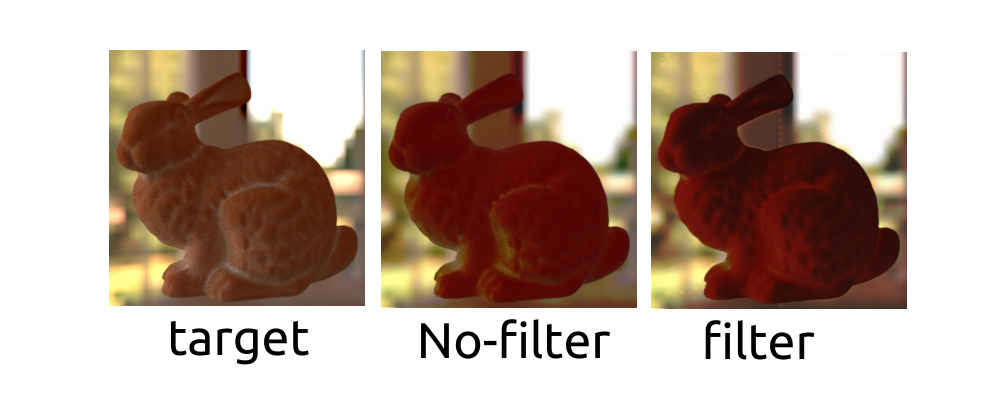
\includegraphics[width=\linewidth]{./figures/result-3.png}
        \centering
        \end{figure}
        \begin{itemize}    
            \item Bias problem, especially lighting by filtered environment map
            \item Bias is accumulated every iteration
        \end{itemize}
    
    % note %
    \note[item] {
    }
\end{frame}

% ==============================================================
% Method : Gradient Descenet Explanations - 3
% ==============================================================   
\begin{frame}{Method}
    \framesubtitle{Result: Gradient filtering on a environment map}
        \begin{figure}[t]
            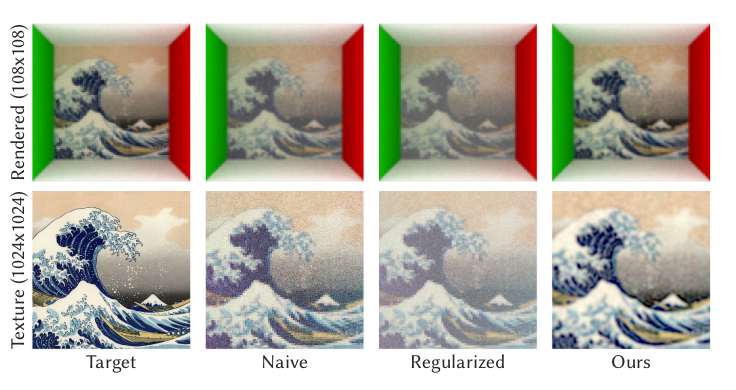
\includegraphics[width=\linewidth]{./figures/result-4.png}
        \centering
        \end{figure}
        \begin{itemize}
            \item Artifacts on lighting by filtered environment map
        \end{itemize}
    % note %
    \note[item] {
    }
\end{frame}

% ==============================================================
% Method : Gradient Descenet Explanations - 2
% ==============================================================   
\begin{frame}{Method}
    \framesubtitle{Result: Gradient filtering on a texture}
        \begin{figure}[t]
            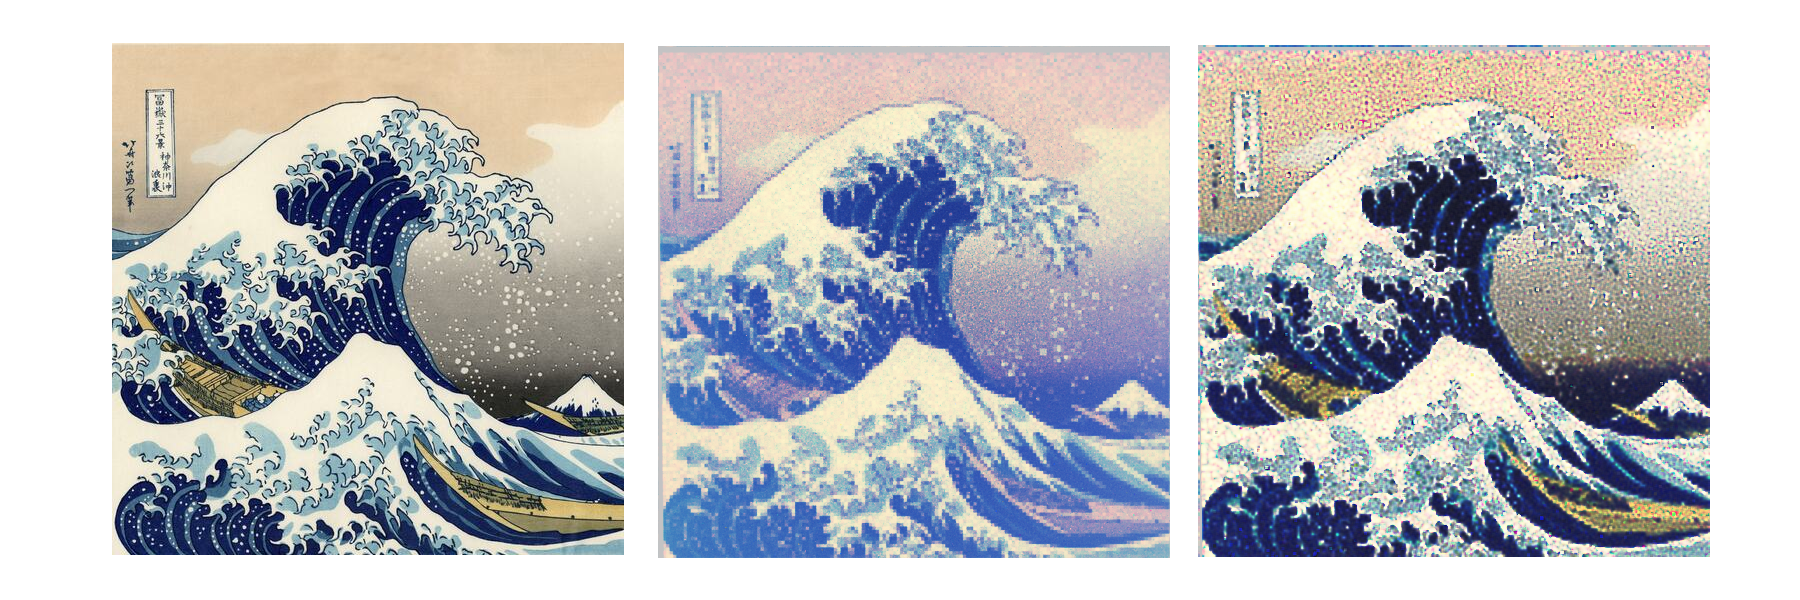
\includegraphics[width=\linewidth]{./figures/result-5.png}
        \centering
        \end{figure}
        \begin{itemize}    
            \item Bias is accumulated every iteration
        \end{itemize}
    
    % note %
    \note[item] {
    }
\end{frame}


\end{document}